% id: 98-01
% book: 베이직쎈 확률과 통계 · 05 확률변수와 확률분포
% section: 실전 감각 UP
% figure: tikz:fig-98-01
% answer: 
% answer_source: 
% variant_level: 0 (원본 전사)
% 이 파일은 build.mjs 가 items.json 에서 만든다. 고칠 때는 items.json 을 고친다.
\smash{\raisebox{1.5mm}{\dmkichul{베이직쎈 확률과 통계 98쪽 01번}}}
다음 그림과 같이 $3$등분한 서로 다른 두 원판에 $1$, $2$, $3$의 숫자가 각각 적혀 있다. 두 원판이 각각 돌다가 멈췄을 때, 두 원판의 바늘이 가리키는 수의 합을 확률변수 $X$라 하자. $X$가 가질 수 있는 값의 개수는? \dmcondfill{바늘이 경계선을 가리키는 경우는 생각하지 않는다.}{}
\par\smallskip\begin{center}\resizebox{\ifdim\width>\linewidth\linewidth\else\width\fi}{!}{% 98-01(인쇄 98쪽) — 3등분한 서로 다른 두 원판과 위쪽의 빨간 바늘. 스캔 삽화라 TikZ 로 다시 그림.
% 두 원판 모두 1(위) · 2(왼쪽 아래) · 3(오른쪽 아래)의 세 칸으로 나뉘어 있고 칸 색만 서로 다르다(원문과 같은 자리·같은 차례).
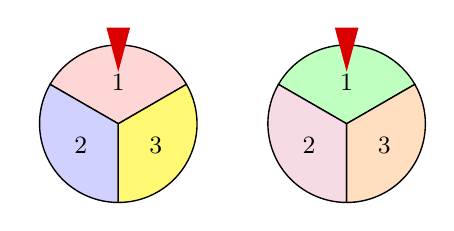
\begin{tikzpicture}[line width=0.5pt, font=\small]
  \def\R{1.0}
  \begin{scope}
    \filldraw[fill=red!16]    (0,0) -- (30:\R)  arc[start angle=30,  end angle=150, radius=\R] -- cycle;
    \filldraw[fill=blue!18]   (0,0) -- (150:\R) arc[start angle=150, end angle=270, radius=\R] -- cycle;
    \filldraw[fill=yellow!55] (0,0) -- (270:\R) arc[start angle=270, end angle=390, radius=\R] -- cycle;
    \node at (90:0.52) {$1$};
    \node at (210:0.55) {$2$};
    \node at (330:0.55) {$3$};
    \fill[red!85!black] (-0.15,1.22) -- (0.15,1.22) -- (0,0.66) -- cycle;
  \end{scope}
  \begin{scope}[shift={(2.9,0)}]
    \filldraw[fill=green!25]  (0,0) -- (30:\R)  arc[start angle=30,  end angle=150, radius=\R] -- cycle;
    \filldraw[fill=purple!14] (0,0) -- (150:\R) arc[start angle=150, end angle=270, radius=\R] -- cycle;
    \filldraw[fill=orange!25] (0,0) -- (270:\R) arc[start angle=270, end angle=390, radius=\R] -- cycle;
    \node at (90:0.52) {$1$};
    \node at (210:0.55) {$2$};
    \node at (330:0.55) {$3$};
    \fill[red!85!black] (-0.15,1.22) -- (0.15,1.22) -- (0,0.66) -- cycle;
  \end{scope}
\end{tikzpicture}
}\end{center}
\dmchoicesauto{}{$3$}{$4$}{$5$}{$6$}{$7$}
